\documentclass[fr]{../../../../../../eplexam}

\usepackage{enumitem}
\newcommand\mean{\mu}
\newcommand\std{\sigma}
\newcommand\var{\std^2}
\newcommand\samplemean[1]{\overline{#1}}
\newcommand\samplestd{S}
\newcommand\samplevar{\samplestd^2}
\DeclareMathOperator{\Gammadist}{Gamma}

\hypertitle{Probabilité et statistiques}{5}{FSAB}{1105}{2018}{Janvier}{All}
{Martin Braquet}
{Anouar El Ghouch et Rainer von Sachs}

\section{QCM (/5)}
Chaque question compte pour 0.5 points, une mauvaise réponse fait perdre 0.25 points et une abstention ne fait pas perdre de point. Puisqu'il y a 11 questions, le résultat est ramené sur 5 points au lieu de 5.5 points. Vous gagnez ainsi un bonus d'un peu moins de 0.5 points.

\subsection{}
On considère deux évènements ayant chacun une probabilité non nulle.

\begin{enumerate}[label=\alph*)]
    \item S'ils ne sont pas mutuellement exclusifs alors ils ne sont pas indépendants.
    \item Ils peuvent être exclusifs et indépendants en même temps.
    \item 
    \item
    \item
    \item 
\end{enumerate}

\subsection{}
On considère un jeu de données de moyenne $\mu$ et de variance $\sigma^2$.

\begin{enumerate}[label=\alph*)]
    \item S'ils ont un écart-type nul, alors toutes les données ont la même valeur.
    \item Si l'écart interquartile est nul, alors au moins 50\% des données sont les mêmes.
    \item La moyenne et l'écart-type ne peuvent être nuls tous les deux.
    \item Si l'espérance et l'écart-type sont tous les deux nuls, alors toutes les données sont les mêmes.
    \item a et b.
    \item a, b et d.
\end{enumerate}

\subsection{}
Nous avonc construit un certain 95\% intervalle de confiance $[a,b]$ pour la moyenne. Que représente cet intervalle?

\begin{enumerate}[label=\alph*)]
    \item 95\% du temps, la moyenne sera comprise entre a et b.
    \item C'est la probabilité que la moyenne empirique se trouve dans l'intervalle 95$\%$ du temps.
    \item Si on génère 100 intervalles avec la formules du CI, 95 d'entre eux contiendront la moyenne $\mu$.
    \item 
    \item Aucune des propositions ci dessus.
    \item 
\end{enumerate}

\subsection{}
Voici 4 images représentant des données $X$ et $Y$, déterminer les coefficients de corrélation de ces échantillons.

\begin{figure}[h!]
    \centering
    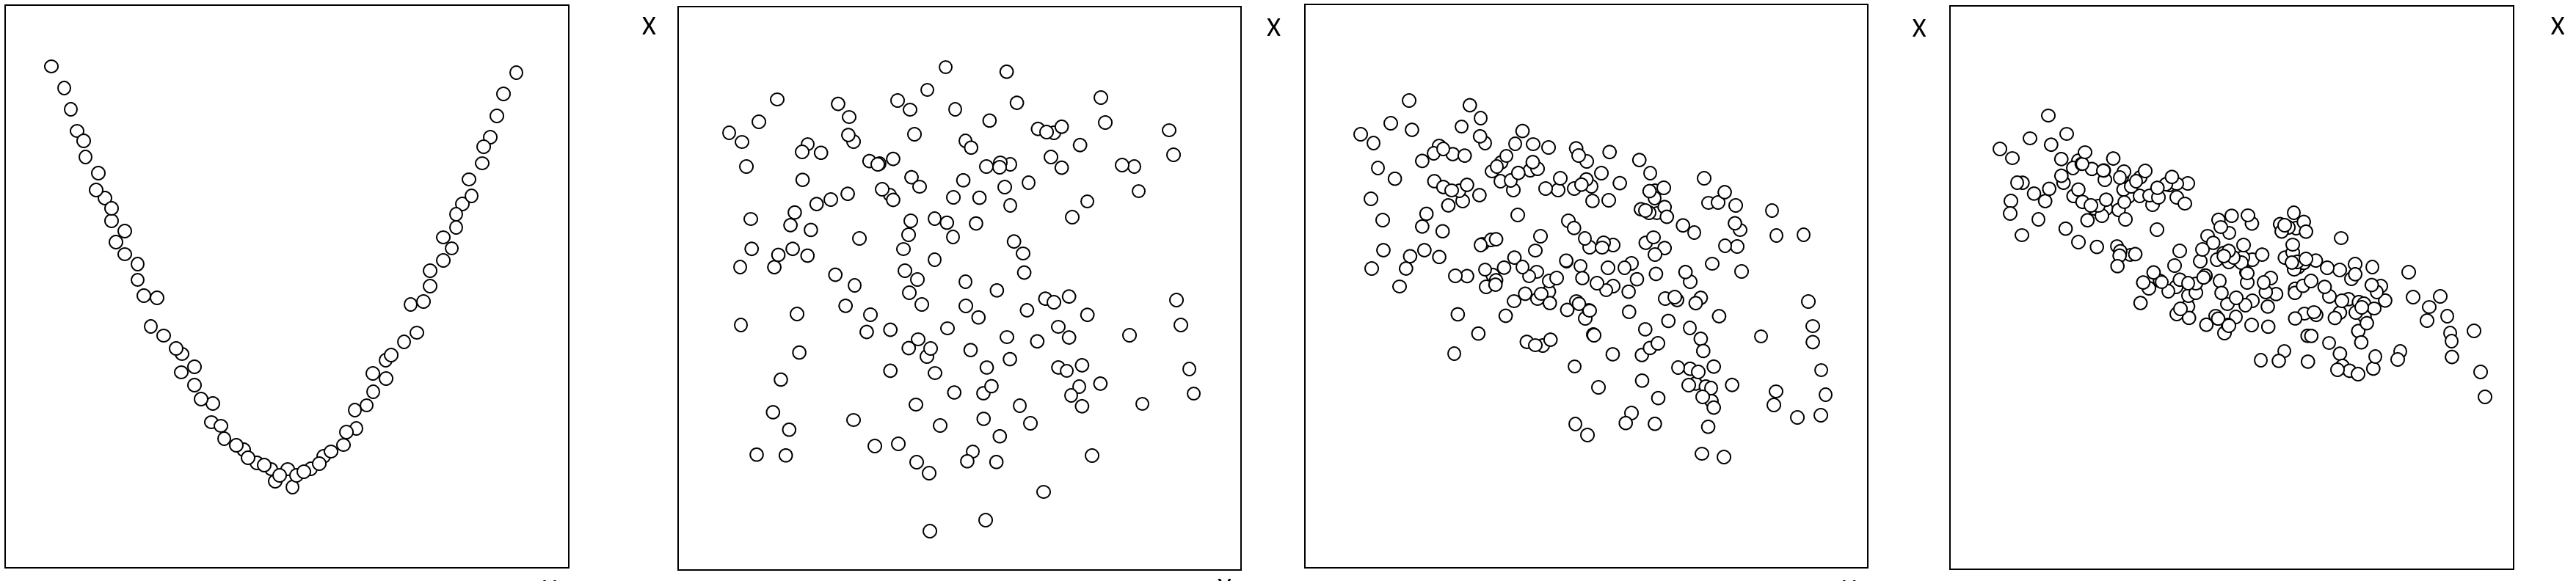
\includegraphics[width=\linewidth]{Jan2018}
\end{figure}

\begin{table}[h!]
\centering
\begin{tabular}{|c|c|c|c|c|}
  \hline
  a) & $\rho_i=0$  & $\rho_{ii}=0$ & $\rho_{iii}=-0.3$ & $\rho_{iiii}=0.8$ \\
  \hline
  b) & $\rho_i=0$  & $\rho_{ii}=1$ & $\rho_{iii}=-0.8$ & $\rho_{iiii}=0.8$ \\
  \hline
  c) & $\rho_i=0$  & $\rho_{ii}=0$ & $\rho_{iii}=-0.3$ & $\rho_{iiii}=-0.8$ \\
  \hline
  d) & $\rho_i=1$  & $\rho_{ii}=-1$ & $\rho_{iii}=0.3$ & $\rho_{iiii}=-0.8$ \\
  \hline
  e) & $\rho_i=1$  & $\rho_{ii}=0$ & $\rho_{iii}=0.8$ & $\rho_{iiii}=-0.8$ \\
  \hline
  f) & $\rho_i=1$  & $\rho_{ii}=1$ & $\rho_{iii}=0.3$ & $\rho_{iiii}=0.8$ \\
  \hline
\end{tabular}
\end{table}

\subsection{}
4 box plots sont représentés sur la figure ci-dessous. Déterminer lequel représente 

\begin{figure}[h!]
    \centering
    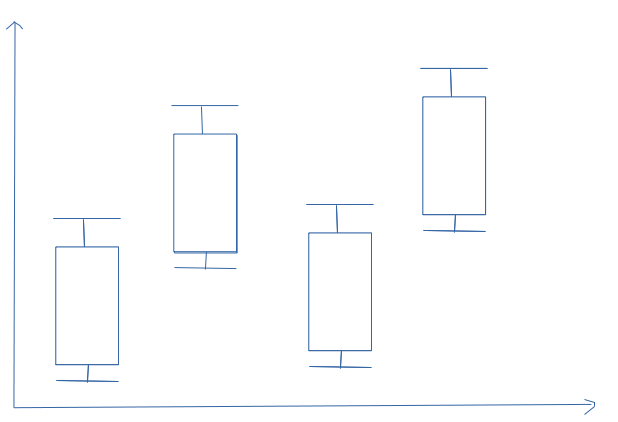
\includegraphics[width=0.6\linewidth]{boxplot}
\end{figure}

\begin{enumerate}[label=\alph*)]
    \item Le box plot des données $X$
    \item Le box plot de: (données $X$) + 2
    \item Le box plot de: 2 $\cdot$ (données $X$)
    \item Le box plot de: 2 $\cdot$ (données $X$) + 2
\end{enumerate}

\subsection{}
Des données sont générées et on en calcule un intervalle de confiance pour la moyenne qui vaut $[1.1;2]$. On réalise ensuite 2 tests d'hypothèse. Le premier est A: $H_0:\mu=1.5$ et $H_1:\mu\neq1.5$, et le second est B: $H_0:\mu=1.3$ et $H_1:\mu>1.3$. Que peut-on dire sur A et B en connaissant l'intervalle de confiance pour la moyenne?

\begin{enumerate}[label=\alph*)]
    \item On ne devrait pas rejeter $H_0$ pour le test A.
    \item On ne devrait pas rejeter $H_0$ pour le test B.
    \item Les données du problème ne permettent pas de conclure sur le test A.
    \item Les données du problème ne permettent pas de conclure sur le test B.
    \item A et C.
    \item A et D.
    \item B et C.
    \item B et D.
    \item Aucune des propositions.
\end{enumerate}

\subsection{}
Des étudiants testent un groupe de 10 personnes pour savoir le nombre d'animaux de compagnie qu'ils possèdent. Pour un groupe $n_1=10$ avec une moyenne $2.35$ et un écart type $0.75$, ils trouvent un intervalle de confiance à 95\% pour la moyenne $IC_1$ de $[1.903,2.795]$. Ensuite, ils testent un échantillon de $n_2=100$, et avec la formule $\overline{X}_{100}\pm 1.96 \: S_{100}/\sqrt{n_2}$, ils trouvent un intervalle $[2.034,2.186]$.
\begin{enumerate}[label=\alph*)]
    \item L'intervalle $IC_1$ est faux, le véritable intervalle est $[1.885,2.815]$.
    \item 
    \item Les 2 intervalles sont correctes.
    \item
    \item
    \item 
\end{enumerate}
Notes : valeurs utilisées arbitraires.

\subsection{}
L'élément suivant n'est pas nécessaire pour calculer une p-valeur.

\begin{enumerate}[label=\alph*)]
    \item Le seuil de signification.
    \item La valeur observée de la statistique de test.
    \item Savoir si le test est unilatéral ou bilatéral.
    \item Plusieurs réponses sont correctes.
    \item Aucune des réponses précédentes n'est correcte.
\end{enumerate}

\begin{solution}

\begin{enumerate}
 \item 
 \item f
 \item c
 \item c
 \item a-1 b-3 c-2 d-4
 \item f
 \item 
 \item a
\end{enumerate}


\end{solution}

\section{(/4)}
Soient les distributions $X$ et $Y$ telles que leur fonction de densité jointe soit égale à 

\[
    f_{X,Y}(x,y)= 15\:yx^2 \qquad \mathrm{si} \qquad 0<x<y<1
\]

\begin{enumerate}
    \item Déterminer $\mathrm{P}( X > \frac{1}{2} \:|\: Y > \frac{1}{2})$.
    \item Soit $U=Y\sqrt{X}$, déterminer la fonction de densité de $U$.
    \item  Déterminer le coefficient de corrélation entre $X$ et $Y$.
    
\end{enumerate}

\begin{solution}

 Voici le domaine de $f_{X,Y}(x,y)$ dans le plan (x,y):
 
\begin{center}
    \begin{tikzpicture}
      \draw[dashed] (2,0) -- (2,2);
      \put(-10,55){$1$}
      \put(55,-10){$1$}
      \fill[fill=gray!50] (0,2)--(0,0)--(2,2);
      \draw[->] (0,0) -- (3,0) node[right] {$x$};
      \draw[->] (0,0) -- (0,3) node[above] {$y$};
      \draw[dashed] (0,2) -- (2,2);
    \end{tikzpicture}
\end{center}

\begin{enumerate}
    \item 
    \[
        \mathrm{P}\left( X > \frac{1}{2} \:|\: Y > \frac{1}{2}\right)  =\frac{\mathrm{P}( X > \frac{1}{2}\cap Y > \frac{1}{2})
        }{\mathrm{P}( Y > \frac{1}{2})}= \frac{\int_{1/2}^1\left( \int_{1/2}^y 15\:yx^2 \mathrm{d}x \right)\:\mathrm{d}y}{\int_{1/2}^1\left( \int_{0}^y 15\:yx^2\mathrm{d}x \right)\:\mathrm{d}y}=0,758
    \]
    \item La première méthode possible est la méthode des transformations. 
    
    On pose $(U,V)=g(X,Y)=(Y\sqrt{X},Y)$ et donc $(X,Y)=g^{-1}(U,V)=\left(\left(\frac{U}{V}\right)^2,V\right)$. On cherche ensuite le domaine de $(U,V)$ par transformation du domaine $(X,Y)$. On sait que $0<v<1$ car $y=v$, que $u>0$ car $y>0$ et $x>0$. Et la condition $y>x$ donne $v>u^{2/3}$. Le domaine est donc
    \[
        0<u<1 \qquad \mathrm{et} \qquad u^{2/3}<v<1
    \]
    
    \begin{center}
    \begin{tikzpicture}
      \draw[->] (0,0) -- (3,0) node[right] {$u$};
      \draw[->] (0,0) -- (0,3) node[above] {$v$};
      \draw [black, thick, scale = 2, domain=0:1.5, samples=50] plot (\x, {(\x)^(2/3)});
      \draw[dashed] (2,0) -- (2,2);
      \put(-10,55){$1$}
      \put(55,-10){$1$}
      \put(90,80){$v=u^{2/3}$}
      \fill [gray!50, scale=2, domain=0:1, variable=\x]
      (0, 1)
      -- plot ({\x}, {(\x)^(2/3)})
      -- (1, 1)
      -- cycle;
    \end{tikzpicture}
\end{center}

    On applique la formule
    \[
        f_{U,V}(u,v)=\left.\frac{f_{X,Y}(x,y)}{|Jac_g(x,y)|} \right|_{(x,y)=g^{-1}(u,v)} 
    \]
    Le jacobien est donné par 
\[
    |Jac_g(x,y)|= \begin{vmatrix}
    \frac{\partial g_1}{\partial x} &\frac{\partial g_1}{\partial y} \\ \frac{\partial g_2}{\partial x} & \frac{\partial g_2}{\partial y} \end{vmatrix} =\begin{vmatrix} \frac{y}{2\sqrt{x}} & \sqrt{x} \\ 0 & 1 \end{vmatrix}=\frac{y}{2\sqrt{x}} \textrm{ car } x,y > 0
\]

On trouve donc que
\[
    f_{U,V}(u,v)=\left.\frac{15\:yx^2}{y/(2\sqrt{x})}\right|_{(x,y)=g^{-1}(u,v)}=\left.30\:x^{5/2}\right|_{x=(u/v)^2}=30\left(\frac{u}{v}\right)^5
\]
La fonction de densité jointe de $U$ vaut ainsi
\[
    f_U(u)=\int_{v^{3/2}}^1 30\left(\frac{u}{v}\right)^5\: \mathrm{d}v=\frac{15}{2}\left(u^{7/3}-u^5\right)\qquad \textrm{si} \qquad 0<u<1.
\]
On peut vérifier que l'intégrale de cette fonction de densité sur son domaine vaut 1.\\

La seconde méthode possible est la méthode des distributions. 

\item 
\begin{align*}
    E[X]&=\int_{0}^1\left( \int_{0}^y x\:f_{X,Y}(x,y) \mathrm{d}x \right)\:\mathrm{d}y=\frac{15}{24}\\
    E[X^2]&=\int_{0}^1\left( \int_{0}^y x^2\:f_{X,Y}(x,y) \mathrm{d}x \right)\:\mathrm{d}y=\frac{15}{35}\\
    E[Y]&=\int_{0}^1\left( \int_{0}^y y\:f_{X,Y}(x,y) \mathrm{d}x \right)\:\mathrm{d}y=\frac{15}{18}\\
    E[Y^2]&=\int_{0}^1\left( \int_{0}^y y^2\:f_{X,Y}(x,y) \mathrm{d}x \right)\:\mathrm{d}y=\frac{15}{21}\\
    E[XY]&=\int_{0}^1\left( \int_{0}^y xy\:f_{X,Y}(x,y) \mathrm{d}x \right)\:\mathrm{d}y=\frac{15}{28}\\
    \rho_{XY}&=\frac{E[XY]-E[X]E[Y]}{\sqrt{\left(E[X^2]-E[X]^2 \right) \left(E[Y^2]-E[Y]^2 \right)}}=0,5423
\end{align*}
\end{enumerate}

\end{solution}

\section{(/3)}
\begin{enumerate}
\item Démontrer que $cU\sim \mathrm{Gamma}(\alpha,c\beta)$ si  $U\sim \mathrm{Gamma}(\alpha,\beta)$.
\item
Soit la variable aléatoire $X$ qui suit une distribution exponentielle d'espérance $\beta$: $X\sim \mathrm{Expo}(\beta)$.
    \begin{enumerate}[label=\alph*)]
    \item On considère $X_1,\ldots, X_n$, des données i.i.d. issues de $X$, démontrer que $Y=\sum_{i=1}^n X_i$ suit une distribution Gamma de paramètres $n$ et $\beta$:  $Y\sim \mathrm{Gamma}(n,\beta)$.
    \item Démontrer que $\frac{2}{\beta}\sum_{i=1}^n X_i$ suit une distribution chi-carré de paramètre $2n$:  $\frac{2}{\beta}\sum_{i=1}^n X_i \sim \chi^2_{2n}$.
    \end{enumerate}
\end{enumerate}
Aide: $\chi^2_{n} \sim \mathrm{Gamma}(n/2, 2)$.

\begin{solution}

\begin{enumerate}
    \item 
    La fonction génératrice de moment de la Gamma est $m_U(t)=(1-\beta t)^{-\alpha}$. La fonction génératrice de moment de $cU$ vaut
    \[
        m_{cU}(t)=E[e^{cUt}]=E[e^{U(ct)}]=m_U(ct)=(1-\beta c t)^{-\alpha},
    \]
    qui est la fonction génératrice de moment de la Gamma$(\alpha,c\beta)$.
    Par équivalence entre distribution et fonction génératrice de moment, la distribution $cU$ suit une Gamma$(\alpha,c\beta)$.
    \item
    \begin{enumerate}[label=\alph*)]
        \item On a
    \[
        m_{Y}(t)=E[e^{Yt}]=E[e^{\sum_i X_i t}]=\prod_i E[e^{X_i t}]=\prod_i m_X(t)=(1-\beta t)^{-n},
    \]
    car les $X_i$ sont indépendants et identiquement distribués. On l'identifie à la fonction génératrice de moment d'une Gamma$(n,\beta)$.
        \item On a
    \[
        m_{\frac{2Y}{\beta}}(t)=E[e^{\frac{2}{\beta} Yt}]=E[e^{ Y(\frac{2t}{\beta})}]=m_Y\left(\frac{2t}{\beta}\right)=(1-2t)^{-n}
    \]
    On l'identifie à la fonction génératrice de moment d'une $\chi^2_\nu$ avec $\nu=2n$ degrés de liberté.
    \end{enumerate}
\end{enumerate}

\end{solution}

\section{Question sur l'APP (/6)}
Soit la variable aléatoire $X$ ayant pour fonction de densité
\[
    f_X(x)=\theta \: x^{\theta-1} \qquad \mathrm{si} \qquad 0<x<1
\]

\begin{enumerate}
    \item Soit $Y = -\ln(X)$. Donner la distribution de $Y$.
    \item Donner l'expression de la médiane de $X$, notée $m$, en fonction de $\theta$.
    \item Soit $X_i$ avec $i=1, ..., n$ un échantillon de variables aléatoires de taille $n$,
        \begin{itemize}
        \item Donner l'estimateur pour $m$ par la méthode des moments.
        \item Donner l'estimateur de maximum de vraisemblance de $m$.
        \item Donner l'intervalle de confiance exact à 95\% pour $m$.
        \item Donner l'intervalle de confiance asymptotique à 95\% pour $m$.
        \end{itemize}
\end{enumerate}

\begin{solution}

\paragraph{Intervalle de confiance pour la moyenne d'une normale}
On considère que $X$ suit une distribution normale d'espérance $\mean$ et de variance $\var$ inconnues.
La médiane d'une distribution normale est $\mean$.
On cherche donc un intervalle $CI_1 = [\hat{a},\hat{b}]$ tel que $ P(\hat{a} \leq \mean \leq \hat{b}) = 1-\alpha$,
avec $\hat{a}$ et $\hat{b}$ ne dépendant que de l'échantillon $X_1,\ldots,X_n$.

Si on note la moyenne de l'échantillon $ \samplemean{X} = \frac{1}{n}\sum_{i=1}^n X_i $
et la variance de l'échantillon $ S^2 = \frac{1}{n-1} \sum_{i=1}^n (X_i - \samplemean{X})^2 $,
alors la variable aléatoire
\[ T = \frac{\samplemean{X} - \mean}{\samplestd/\sqrt{n}} \]
suit une distribution de Student à $n-1$ degrés de liberté.
On peut donc trouver dans les tables $t_{\alpha/2}$ et $t_{-\alpha/2}$ tels que
\[ P(-t_{\alpha/2} \leq T \leq t_{\alpha/2}) = 1-\alpha. \]

En manipulant les inégalités, on trouve l'intervalle de confiance pour $\mean$:
\[ CI_1 = \left[
    \samplemean{X} - \frac{\samplestd}{\sqrt{n}} t_{n-1,\alpha/2};
    \samplemean{X} + \frac{\samplestd}{\sqrt{n}} t_{n-1,\alpha/2}
\right] \]

\paragraph{Intervalle de confiance pour la médiane d'une distribution continue donnée}
On considère que $X$ possède la fonction de densité suivante
\[ f(x) = \beta x^{\beta-1} \:I[0 < x < 1] \]
avec $ \beta > 0 $ inconnu.
Sa fonction de distribution cumulative s'exprime
\[ F(x) = x^\beta\: I[0 < x < 1] + I[x \geq 1] \]
Soit la variable aléatoire $ Y = -\log(X) $.
On trouve sa fonction de distribution cumulative $G(y)$
\begin{align*}
    G(y)    &= P(Y \leq y) = P(-\log(X) \leq y) =  P(X \geq e^{-y}) = 1 - P(X \leq e^{-y}) \\
            &= 1 - F(e^{-y}) = (1-e^{-\beta y}) \:I[y > 0]
\end{align*}
et sa fonction de densité $ g(y) = G'(y) = \beta e^{-\beta y} \:I[y > 0] $.
La variable $Y$ suit donc une \emph{distribution exponentielle}
d'espérance $ \mean_Y = 1/\beta $ et de variance $ \var_Y = 1/\beta^2 $.

La médiane $m$ de $X$ s'obtient en résolvant
\[ F(m) = \frac{1}{2} \quad\Rightarrow\quad m = 2^{-1/\beta}. \]
Trouver un intervalle de confiance pour $m$ se réduit donc à trouver un intervalle de confiance pour $ \beta $.

\paragraph{Intervalle de confiance exact pour $m$}
Soit $Y_1,\ldots,Y_n$ l'échantillon tel que $ Y_i = -\log{X_i} $.
Par la propriété 2 dans l'énoncé, $ \sum_i Y_i = n\samplemean{Y} \sim \Gammadist(n,1/\beta) $
et par les propriétés 3 et 4, $ 2\beta n \samplemean{Y} \sim \Gammadist(n,2) = \chi_{2n}^2 $.
On peut donc trouver dans les tables $\chi_{2n,1-\alpha/2}$ et $\chi_{2n,\alpha/2}$
tels que
\[
    P\left(\chi_{2n,1-\alpha/2}^2 \leq 2\beta n \samplemean{Y} \leq \chi_{2n,\alpha/2}^2\right) = 1-\alpha
\]
où $\chi^2_{\nu,p}$ est le quantile d'ordre $1-p$ d'une distribution $\chi^2$ à $\nu$ degrés de liberté.

En manipulant les inégalités, on trouve un intervalle de confiance pour $\beta$:
\[ CI_\beta = \left[
    \frac{\chi^2_{2n,1- \alpha/2}}{2n\samplemean{Y}};
    \frac{\chi^2_{2n, \alpha/2}}{2n\samplemean{Y}}
\right]. \]
Sachant que $ n\samplemean{Y} = \sum_i{Y_i} = \sum_i{-\log{X_i}} = -\log{\prod_i{X_i}} $
et en utilisant la loi de transformation des intervalles de confiance pour $ m = 2^{-1/\beta} $
(fonction croissante pour $ \beta > 0 $), on trouve
\[ CI_2 = \left[
    \left(\textstyle{\prod_i{X_i}}\right)^{2\log{2} / \chi^2_{2n,1- \alpha/2}} ;
    \left(\textstyle{\prod_i{X_i}}\right)^{2\log{2} / \chi^2_{2n,\alpha/2}}
\right]. \]

\paragraph{Intervalle de confiance asymptotique pour $m$}
Si $n$ est suffisamment grand, alors le théorème central limite
 dit que $ \samplemean{Y} $ suit une distribution normale
de moyenne $ \mean_Y = 1/\beta $ et de variance $ \var_Y/n = 1/(\beta^2 n) $:
\[ \samplemean{Y} \sim N \left( \frac{1}{\beta}, \frac{1}{\beta^2 n} \right). \]
On peut donc trouver dans les tables $ z_{\alpha/2} $ tel que
\[ P\left(
    -z_{\alpha/2} \leq \frac{\samplemean{Y}-1/\beta}{1/(\beta\sqrt{n})} \leq z_{\alpha/2}
\right) = 1-\alpha \]
Pour $\alpha=0.05$, on a $z_{\alpha/2}=1.96$.
En manipulant les inégalités, on trouve un intervalle de confiance pour $ \beta $:
\[ CI_\beta = \left[
    \frac{1 - z_{\alpha/2}/\sqrt{n}}{\samplemean{Y}} ;
    \frac{1 + z_{\alpha/2}/\sqrt{n}}{\samplemean{Y}}
\right]. \]
Par une transformation similaire à celle effectuée pour trouver $CI_2$, on trouve
\[ CI_3 = \left[
    \left(\textstyle{\prod_i{X_i}}\right)^{\log{2}/ (n - \sqrt{n} z_{\alpha/2})} ;
    \left(\textstyle{\prod_i{X_i}}\right)^{\log{2}/ (n + \sqrt{n} z_{\alpha/2})}
\right]. \]

\end{solution}

\section{Qui mange le plus de choux? (/2)}
Un concours du plus grand mangeur de choux est organisé, on veut déterminer si les hommes en mangent en moyenne plus que les femmes. Les résultats du test sur 10 hommes ($Y_1$) et 9 femmes ($Y_2$) sont donnés dans la table ci-dessous. $\mu_1$ et $\mu_2$ représentent respectivement la moyenne de la masse de choux mangée par un homme et par une femme (en kg). Faites un test statistique pour déterminer si, en moyenne, les hommes mangent plus de choux que les femmes. Considérez $\alpha=0.5\%$.
Quels sont les hypothèses que vous avez faites pour faire votre test? Que pouvez-vous en conclure? Donnez l'expression de la p-valeur (2 bornes).

\begin{table}[h!]
\centering
\begin{tabular}{|c|c|c|c|c|c|c|c|c|c|c|}
  \hline
  $Y_1$ & 2,09  & 2.49 & 1.98 & 3.2 & 2.56 & 1.99 & 2.64 & 2.77 & 2.69  & 2.25 \\
  \hline
  $Y_2$ & 2.5 & 2.06 & 1.65 & 1.01 & 2.35 & 1.88 & 1.89 & 2.28 & 2.23 & \\
  \hline
\end{tabular}
\end{table}

\nosolution

\end{document}
